\pgfdeclarelayer{tracks}
\pgfsetlayers{tracks,main}
\tikzset{
    tracks/.style={
        postaction={draw=gray,densely dashed,line width=12pt},
        postaction={draw=black,double distance=5pt,line width=2pt},
        postaction={draw=gray,densely dashed,line width=5pt},
        shorten <=-5pt, shorten >=-5pt
    },
    crossing/.style={
        circle,
        minimum size=18pt,
        draw,
        fill=white,
        ultra thick
    },
    sidingstore/.style={
        rectangle,
        draw,
        ultra thick,
        fill=white,
        minimum width=6mm,
        minimum height=6mm,
        label position={#1},
        label distance=2mm
    },
    siding/.style 2 args={
        style=crossing,
        label=[{sidingstore={#2}}]{\scriptsize\textbf{#1}},
        prefix after command={\pgfextra{\path [tracks] ($(\tikzlastnode)$) to ($(\tikzlastnode)+(#2:5mm)$);}}
    },
    station/.style={
        label={center: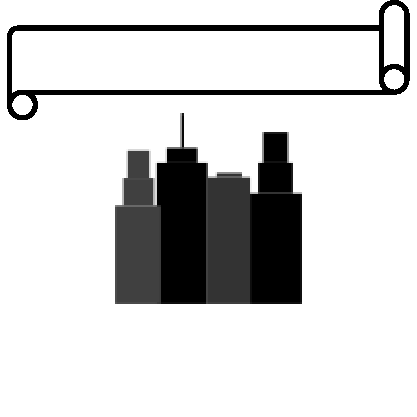
\includegraphics[scale=0.35]{../../src/main/resources/city}},
        label={[label distance=4.5mm]above:{\scriptsize\strut #1}}
    }
}
